% Mohan's CARLA figure revision, 2026-11-17.
% Keep this input and figures/carla_main_20261117 when syncing from the code repository.
% Height is capped at the previous placeholder's aspect ratio to preserve the page budget.
\begin{figure*}[t]
  \centering
  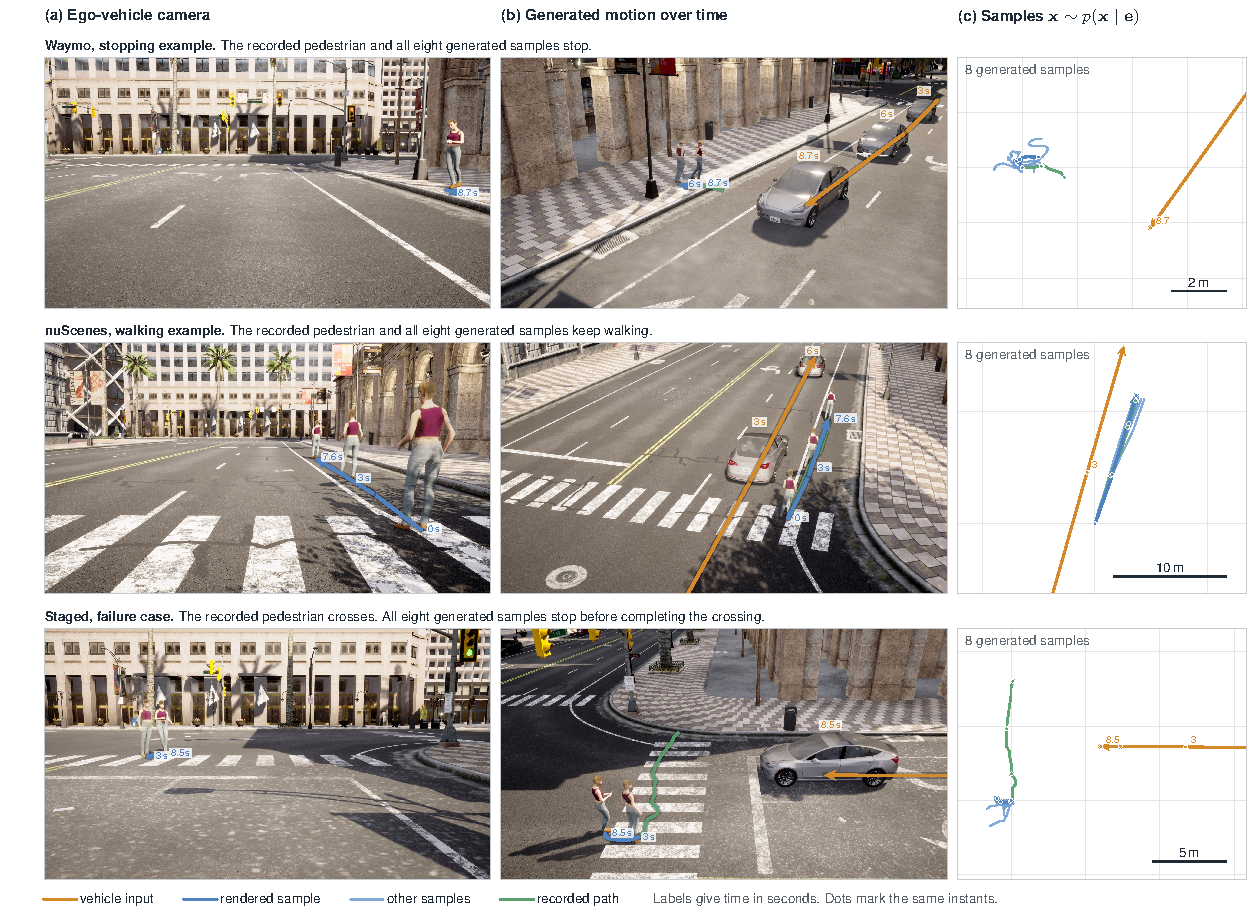
\includegraphics[width=\linewidth,height=0.6053\linewidth,keepaspectratio]{figures/carla_main_20261117/figure.pdf}
  \caption{Generated motion from three test conditions is retargeted to CARLA~\cite{dosovitskiy2017carla} without learned refinement. Each row shows a fixed vehicle-view camera, an elevated temporal composite and the root paths of all eight samples in a metric bird's-eye view aligned with the elevated camera. The rendered sample is the root-path medoid. Time labels are in seconds and overlapping exposures are omitted. Rows one and three are mirrored jointly with the vehicle. The recording is one possible outcome, not a reconstruction target. Pose artifacts remain (Section~\ref{sec:posequality}).}
  \label{fig:qualitatives}
\end{figure*}
